\documentclass[10pt, twocolumn]{article}
\usepackage{authblk} % \affil
\usepackage[utf8]{inputenc}
%Gummi|065|=)

\title{\vspace{-2cm}\textbf{Theoretical Guide\\Lenhadoras de Segtree}}
\author{Nathália Pereira, Duda Holanda $\&$ Duda Carvalho}
\date{}

\usepackage[english]{babel}
\usepackage[utf8]{inputenc}
\usepackage{lscape}
\usepackage[T1]{fontenc}
\usepackage{fancyhdr}
\usepackage{rotating}
\usepackage{ragged2e}
\usepackage[a4paper, landscape, margin=0.8in]{geometry}
\usepackage{blindtext}
\usepackage{amsmath}
\usepackage{relsize}
\usepackage{graphicx}
\usepackage{float}
\usepackage{placeins}
\usepackage{enumitem}
\usepackage{booktabs}
\usepackage{array}
\usepackage{xcolor,colortbl}
\usepackage{tabu}
\usepackage{url}
\usepackage{textcomp}
\usepackage{diagbox}
\usepackage{caption}
\usepackage{amsfonts}
\usepackage{amsmath}
\usepackage{listings} % code
\usepackage{mathtools} % DeclarePairedDelimiter

\lstdefinestyle{c++}{
    language=C++,
    basicstyle=\footnotesize\ttfamily,
    tabsize=2,
    breaklines=true,
    escapeinside={@}{@},
    showstringspaces=false,
    morekeywords={ll},
    breakatwhitespace=false,
    captionpos=b,
    keepspaces=true,
    numbers=left,
    numbersep=5pt,
    showspaces=false,
    showstringspaces=false,
    showtabs=false,
    extendedchars=false,
    inputencoding=utf8,
}

\usepackage{hyperref}
\hypersetup{
    colorlinks=true,
    linkcolor=blue,
    filecolor=magenta,      
    urlcolor=blue,
}

%color celula da tabela
\usepackage{xcolor,colortbl}

\setlength{\columnseprule}{0.4pt}
\setlength{\columnsep}{3em}
\graphicspath{ {img/} }
\restylefloat{table}

\newcommand{\mc}[2]{\multicolumn{#1}{c}{#2}}
\definecolor{Gray}{gray}{0.85}
\newcolumntype{a}{>{\columncolor{Gray}}c}

\newcommand{\stirlingfirst}[2]{\genfrac{[}{]}{0pt}{}{#1}{#2}}
\newcommand{\stirlingsecond}[2]{\genfrac{\{}{\}}{0pt}{}{#1}{#2}}
\newcommand{\lcm}{\mathrm{lcm}}
\DeclarePairedDelimiter\ceil{\lceil}{\rceil}
\DeclarePairedDelimiter\floor{\lfloor}{\rfloor}

\pagestyle{fancy}

\begin{document}
\maketitle
\tableofcontents\section{Number Theory}
$$ (a + b) \text{ mod } m = (a \text{ mod } m + b \text{ mod } m) \text{ mod } m $$
$$ (a - b) \text{ mod } m = (a \text{ mod } m - b \text{ mod } m) \text{ mod } m $$
$$ (a \times b) \text{ mod } m = ((a \text{ mod } m) \times (b \text{ mod } m)) \text{ mod } m $$
$$ a^b \text{ mod } m = (a \text{ mod } m)^b \text{ mod } m $$
$$ a \equiv b \text{ } (\text{mod } m) \iff (b - a) \vert m $$

$$ \gcd(a_1, a_2, a_3, a_4) = \gcd(a_1, \gcd(a_2, \gcd(a_3, a_4))) $$
$$ \lcm(a, b) \times \gcd(a, b) = a \times b $$
$$ \lcm(a, b) = \dfrac{a \times b}{\gcd(a, b)} = \dfrac{a}{\gcd(a,b)} \times b $$
$$ gcd(a, b) = b ? gcd(b, a \% b) : a $$
\subsection{Fermat's Theorems}
Let P be a prime number and $a$ an integer, then:
$$a^p \equiv a \quad (\text{mod } p)$$
$$a^{p-1} \equiv 1 \quad (\text{mod } p)$$

\textbf{Lemma:} Let $p$ be a prime number and $a$ and $b$ integers, then: 
$$(a+b)^{p} \equiv a^{p} + b^{p} \quad (\text{mod } p)$$

\textbf{Lemma:} Let $p$ be a prime number and $a$ an integer. The inverse of $a$ modulo $p$ is $a^{p-2}$:

$$a^{-1} \equiv a^{p-2} \quad (\text{mod } p)$$
\subsection{Prime counting function - \texorpdfstring{$\pi(x)$}{}}

Expected to have $ \frac{x}{\log{x}} $ primes within $[1, x]$. The prime counting function is asymptotic to $\frac{x}{\log x}$, by the prime number theorem.

\ 

\begin{tabular}{|c|c|c|c|c|c|c|c|c|}
\hline
  \cellcolor{gray!40} x&10&$10^2$&$10^3$&$10^4$&$10^5$&$10^6$&$10^7$&$10^8$\\ \hline
  \cellcolor{gray!40} $\pi(x)$& 4 & 25 & 168 & 1\,229 & 9\,592 & 78\,498 & 664\,579 & 5\,761\,455\\ \hline
\end{tabular}

\ 
\subsection{Number of digits of n in base b}
If
$$
\sqrt[k]{n} < b  
$$
then n has k or less digits when written in base b.

\subsection{Number of Divisors}

The number of divisors of $n$ is about $\sqrt[3]{n}$.

\begin{table}[H]
    \centering
    \begin{tabular}{|c|c|c|c|c|c|c|c|c|c|c|c|c|}
        \hline
        \cellcolor{gray!40} $n$ & 6 & 60 & 360 & 5040 & 55440 & 720720 & 4324320 & 21621600 \\
        \hline
        \cellcolor{gray!40} $d(n)$ & 4 & 12 & 24 & 60 & 120 & 240 & 384 & 576 \\
        \hline
    \end{tabular}
\end{table}
\subsection{Sum of digits of n in base b}
$$
f(n, b) = \begin{cases}
    n & n < b\\
    f \left( n, \floor*{\dfrac{n}{b}} + (n \mod b) \right) & n \geq b \\
\end{cases}
$$

\subsection{Number of digits of n! in base b}
$$ \log _{b} n! = \log _{b} (1 \times 2 \times 3 \times ... \times n) = \log _{b} 1 + \log _{b} 2 + \log _{b} 3 + ... + \log _{b} n $$
\section{C++}
\subsection{Priority Queue}
\begin{lstlisting}[language=C++]
template<class T> using min_priority_queue =
priority_queue<T, vector<T>, greater<T>>;
\end{lstlisting}
\subsection{Ordered set and multiset}

\begin{lstlisting}[language=C++]
typedef tree<pair<ll, ll>, null_type, less<pair<ll, ll>>,
rb_tree_tag, tree_order_statistics_node_update> ordered_set;
\end{lstlisting}

\noindent To change to multiset switch equal to less\_equal.
\section{Bitwise}
\subsection{NOT}

\begin{table}[H]
    \centering
    \begin{tabular}{|c|c|}
        \hline
        \cellcolor{gray!40} $A$ & \cellcolor{gray!40} $X$ \\
        \hline
        0 & 1 \\
        \hline
        1 & 0 \\
        \hline
    \end{tabular}
\end{table}

\subsection{AND}

\begin{table}[H]
    \centering
    \begin{tabular}{|c|c|c|}
        \hline
        \cellcolor{gray!40} $A$ & \cellcolor{gray!40} $B$ & \cellcolor{gray!40} $X$ \\
        \hline
        0 & 0 & 0 \\
        \hline
        0 & 1 & 0 \\
        \hline
        1 & 0 & 0 \\
        \hline
        1 & 1 & 1 \\
        \hline
    \end{tabular}
\end{table}

\subsection{OR}

\begin{table}[H]
    \centering
    \begin{tabular}{|c|c|c|}
        \hline
        \cellcolor{gray!40} $A$ & \cellcolor{gray!40} $B$ & \cellcolor{gray!40} $X$ \\
        \hline
        0 & 0 & 0 \\
        \hline
        0 & 1 & 1 \\
        \hline
        1 & 0 & 1 \\
        \hline
        1 & 1 & 1 \\
        \hline
    \end{tabular}
\end{table}

\subsection{NAND}

\begin{table}[H]
    \centering
    \begin{tabular}{|c|c|c|}
        \hline
        \cellcolor{gray!40} $A$ & \cellcolor{gray!40} $B$ & \cellcolor{gray!40} $X$ \\
        \hline
        0 & 0 & 1 \\
        \hline
        0 & 1 & 1 \\
        \hline
        1 & 0 & 1 \\
        \hline
        1 & 1 & 0 \\
        \hline
    \end{tabular}
\end{table}

\subsection{NOR}

\begin{table}[H]
    \centering
    \begin{tabular}{|c|c|c|}
        \hline
        \cellcolor{gray!40} $A$ & \cellcolor{gray!40} $B$ & \cellcolor{gray!40} $X$ \\
        \hline
        0 & 0 & 1 \\
        \hline
        0 & 1 & 0 \\
        \hline
        1 & 0 & 0 \\
        \hline
        1 & 1 & 0 \\
        \hline
    \end{tabular}
\end{table}

\subsection{XOR}

\begin{table}[H]
    \centering
    \begin{tabular}{|c|c|c|}
        \hline
        \cellcolor{gray!40} $A$ & \cellcolor{gray!40} $B$ & \cellcolor{gray!40} $X$ \\
        \hline
        0 & 0 & 0 \\
        \hline
        0 & 1 & 1 \\
        \hline
        1 & 0 & 1 \\
        \hline
        1 & 1 & 0 \\
        \hline
    \end{tabular}
\end{table}

\subsection{XNOR}

\begin{table}[H]
    \centering
    \begin{tabular}{|c|c|c|}
        \hline
        \cellcolor{gray!40} $A$ & \cellcolor{gray!40} $B$ & \cellcolor{gray!40} $X$ \\
        \hline
        0 & 0 & 1 \\
        \hline
        0 & 1 & 0 \\
        \hline
        1 & 0 & 0 \\
        \hline
        1 & 1 & 1 \\
        \hline
    \end{tabular}
\end{table}
\subsection{XOR from 1 to n}
$$
f(n) = \begin{cases}
    n & n \equiv 0\ (\text{mod } 4)\\
    1 & n \equiv 1\ (\text{mod } 4)\\
    n+1 & n \equiv 2\ (\text{mod } 4)\\
    0 & n \equiv 3\ (\text{mod } 4)\\
\end{cases}
$$

\subsection{Number of bits on}
__builtin_popcount(x)
\subsection{Count leading zeros}
__builtin_clz(z)
__builtin_clzll(z)
\subsection{MSB}
32 - _builtin_clz(x)
64 - __bultin_clzll(x)
\subsection{Count trailing zeros}
__builtin_ctz(x)
__builtin_ctzll(x)
\subsection{LSB}
__builtin_ffs(X)

\subsection{Turn bit on and off}
Turn on bit i \lstinline{x & (1 << i)}\\
Turn off bit i \lstinline{x & (~(1 << i))}\\
\section{Constants}
\begin{lstlisting}[language=C++]
LLINF = 0x3f3f3f3f3f3f3f3fLL
\end{lstlisting}

\begin{lstlisting}[language=C++]
PI = acos(-1)
\end{lstlisting}

\section{Progressions}
\subsection{Geometric Progression}
\subsubsection{General Term}
$$ a_{1} q^{n - 1} $$
\subsubsection{Sum}
$$ \dfrac{a_{1} (q^{n} - 1)}{q - 1} $$
\subsubsection{Infinite Sum}
$$ -1 < q < 1 $$
$$ \dfrac{a_{1}}{1 - q} $$
\subsection{Arithmetic Progression}
\subsubsection{General Term}
$$ a_{1} + (n - 1) r $$
\subsubsection{Sum}
$$ \dfrac{(a_{1} + a_{n}) n}{2} $$
\subsubsection{Sum of Second Order Arithmetic Progression}
$a_{1}$ is the first element of the original progression, $b_{1}$ is the first element of the derived progression, $n$ is the number of elements of the original progression and $r$ is the ratio of the derived progression
$$ a_{1} n + \dfrac{(b_{1} n (n - 1)}{2} + \dfrac{r n (n - 1) (n - 2)}{6} $$
\section{Basic Math}
\subsection{Logarithm}

$$ \log _{b} mn = \log _{b} m + \log _{b} n \quad\quad log _{b} \dfrac{m}{n} = \log _{b} m - \log _{n} n \quad\quad \log _{b} n^p = p \log _{b} n$$
$$ \log _{b} \sqrt[q]{n} = \dfrac{1}{q} \log _{b} n \quad\quad \log _{b} n = \log _{a} n \log _{b} a \quad\quad b^{\log _{b} k} = k $$
$$ \log _{b} a = \dfrac{\log _{c} a}{\log _{c} b} \quad\quad \log _{b} a = \dfrac{1}{\log _{a} b} \quad\quad \log _{b} a \text{ } \log _{a} c = \log _{b} c $$
$$ \log _{b} 1 = 0 \quad\quad \log _{b} b = 1 $$
\subsection{Divisibility Criteria}
\subsubsection{2}
The last digit is either 0, 2, 4, 6 or 8
\subsubsection{3}
The sum of the digits is also divisible by 3
\subsubsection{4}
The last two digits form a number that is divisble by 4
\subsubsection{5}
The last digit is either 0 or 5
\subsubsection{6}
It has to be divisible by both 2 and 3
\subsubsection{7}
The subtraction of the number formed without the last digit and the last digit times 2 is also divisible by 7
\subsubsection{8}
The last three digits form a number that is divisble by 8
\subsubsection{9}
The sum of the digits is also divisible by 9
\section{Combinatorics}
\subsection{Burnside's Lemma}
Burnside’s lemma can be used to count the number of combinations so that
only one representative is counted for each group of symmetric combinations.
For example, if we have a necklace with different colored pearls and we want to know
how many different combinations we can make.

For example, if we have a necklace colored like this:

\begin{center}
    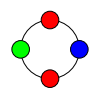
\includegraphics[scale=.6, keepaspectratio]{./Theory/images/burnside1.png}
\end{center}

This variations are the same if we consider that we can rotate the necklace:

\begin{center}
    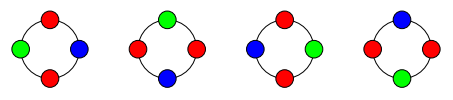
\includegraphics[scale=.6, keepaspectratio]{./Theory/images/burnside2.png}
\end{center}

When the number of steps is k, the number of necklaces that remain the same are:
$$ m^{gcd(k, n)} $$

The number of diferent combinations for m colors and a necklace of size n is 
$$ \sum_{i=0}^{n - 1} \dfrac{m^{gcd(i, n)}}{n} $$

So a necklace of length 4 with 3 colors has
$$ \dfrac{3^{4} + 3 + 3^{2} + 3}{4} = 24 $$
\section{Misc}
\subsection{Check for overflow}
long long v;
// false if no overflow
// true if overflow
__builtin_add_overflow(a, b, v);
cout << v << '\n'; // result of sum

__builtin_sub_overflow(a, b, v);
__builtin_mul_overflow(a, b, v);

\subsection{Input by file}

freopen("input.txt","r",stdin);

\noindent freopen("output.txt","w",stdout);

\section{Geometry}
\subsection{Triangle Existence Condition}
$$a + b \geq c$$
$$a + c \geq b$$
$$b + c \geq a$$
\subsection{Distances}
\subsubsection{Euclidean}
$$ d(p,q)={\sqrt {(q.x-p.x)^{2}+(q.y-p_.y)^{2}}} $$
\subsubsection{Manhattan}
$$ |p.x - q.x| + |p.y - q.y| $$
\subsection{Maximum possible manhattan distance between two points given n points}
Given n points, for instance:
\begin{center}
    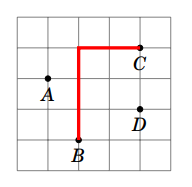
\includegraphics[scale=.6, keepaspectratio]{./Theory/images/manhattan_before.png}
\end{center}

Rotate all coordinates $45^{o}$ do that $(x, y)$ becomes $(x+y, y-x)$, so, $p$ becomes $p'$ and $q$ becomes $q'$.
\begin{center}
    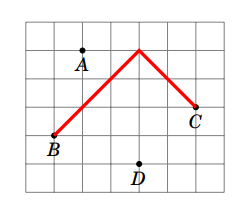
\includegraphics[scale=.6, keepaspectratio]{./Theory/images/manhattan_after.png}
\end{center}

The maximum manhattan distance is obtaining by choosing the two points that maxime:
$$ max(|p'.x - q'.x|, |p'.y - q'.y|) $$
\subsection{Sines Rule}
$$ \dfrac{a}{sin(\alpha)} = \dfrac{b}{sin(\beta)} = \dfrac{c}{sin(\gamma)} $$

\subsection{Cossines Rule}
$$ a^2 = b^2 + c^2 - 2bccos(\alpha) $$
\subsection{Pick's Theorem}
$$ A = a + \dfrac{b}{2} - 1 $$

where $A$ is the area of the polygon, $a$ is the number of integer points inside the polygon and $b$ is the number of integer points in the boundary of the polygon (not counting the vertexes).

\subsection{Boundary points}
The number of integer points in the boundary of a polygon is:
$$ B = v + b $$
where v is the number of vertices (integer points as well) and b is the number of integer points situated between two vertices,
like in the following figure:

\begin{center}
    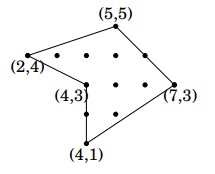
\includegraphics[scale=.6, keepaspectratio]{./Theory/images/pick.png}
\end{center}

b can be calculated for every line connecting two points (including the line between the last and the first point) as follows:

$$
boundary\_points(p, q) = \begin{cases}
    |p.y - q.y| - 1 & $p.x = q.x$\\
    |p.x - q.x| - 1 & $p.y = q.y$\\
    gcd(|p.x - q.x|, |p.y - q.y|) - 1 \\
\end{cases}
$$
\subsection{Perimeter}
\subsubsection{Circle}
$$ 2 \pi r $$

\subsection{Areas}
\subsubsection{Circle}
$$ \pi r^2 $$
\subsubsection{Triangle}
$$ \dfrac{b * h}{2} $$
\subsubsection{Square}
$$ l^2 $$
\subsubsection{Rectangle}
$$ hr $$
\subsubsection{Rhombus}
\begin{center}
    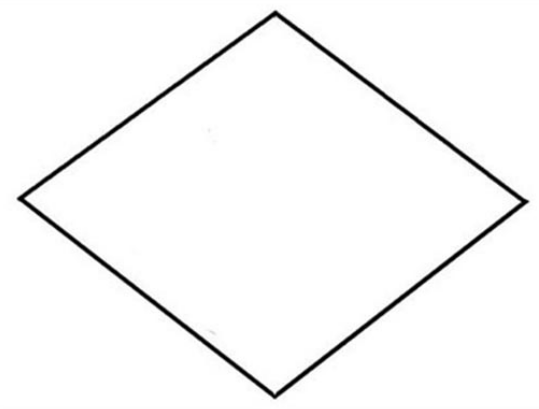
\includegraphics[scale=.2, keepaspectratio]{./Theory/images/rhombus.png}
\end{center}
$D$ is the biggest diagonal and $d$ is the smallest diagonal
$$ A = \dfrac{1}{2} * D * d $$

\subsection{Volumes}
\subsubsection{Sphere}
$$ \dfrac{4}{3} \pi r^3 $$
\subsubsection{Prism}
$$ V = b h $$
\subsubsection{Pyramid}
$$ \dfrac{bh}{3} $$
\subsubsection{Cone}
$$ \dfrac{\pi r^2 h}{3} $$

\subsection{Shoelace Formula}
Calculates the area of a polygon.

$$ A = \dfrac{1}{2} | \sum_{i=1}^{n - 1} (p_{i} \times p_{i+1}) = \dfrac{1}{2} | \sum_{i=1}^{n - 1} (x_{i} y_{i+1} - x_{i+1} y_{i}) | $$

Where the points $p_{1}, p{n}, \dots$ are in adjecent order and the first and last vertex is the same, that is, $p_{1} = p{n}$

\section{Identities}
$$ \sum_{i=1}^{n} i = \dfrac{n(n+1)}{2} \qquad \sum_{i=1}^{n} i^{2} = \frac{n(n+1)(2n+1)}{6} \qquad \sum_{i=1}^{n} i^{3} = \left( \dfrac{n(n + 1)}{2} \right)^2 $$
$$ \sum_{i=1}^{n} \dfrac{1}{i} \approx \log{n} \qquad \sum_{i=0}^{\infty} \dfrac{1}{2^i} = 2 $$


\end{document}
